\chapter{Bayesian Optimization}
\label{chapter:bo}

In this chapter we explore Bayesian optimization from a higher level perspective. We describe the steps of the algorithm and give more motivation for choosing GPs as a probabilistic model. We also explain the difference between hyperparameter tuning and architecture search, which, even though similar at first, are completely different tasks. Lastly, we present some examples of related work, both from the point of hyperparameter tuning, as well as related areas, such as \cite{automl}.

Consider the problem of optimizing an arbitrary continuous function $f: 𝓧 → ℝ$
where $𝓧 ⊂ ℝ^d, d ∈ ℕ$. We call $f$ the \emph{objective function} and treat it
as a black box, making no other assumptions on its analytical form, or on our
ability to compute its derivatives. Our goal is to find the global minimum
$\vx_\text{opt}$ over the set $𝓧$, that is
$$
\vx_\text{opt} = \argmin_{\vx ∈ 𝓧} f(\vx).
$$

We also assume that the evaluation of $f$ is expensive, as the goal of Bayesian
optimization is to find the optimum in as few evaluations as possible. Consider
the case when evaluating $f$ means performing a computation that is not only
time consuming, but for example also costs a lot of money. We might only have a
fixed budget which puts a hard limit on the number of evaluations we can
perform. If the function can be evaluated cheaply, other global optimization
approaches such as simulated annealing or evolution strategies could
potentially yield better results \citep{google-vizier}.

Bayesian optimization techniques are some of the most efficient approaches in
terms of the number of function evaluations required. Much of the efficiency
stems from the ability to incorporate prior belief about the problem and to
trade of exploration and exploitation of the search space
\citep{nando-bopt-tutorial}.

It is called Bayesian because it combines the prior knowledge $p(f)$ about the
function together with the data in the form of the likelihood $p(x|f)$ to
formulate a posterior distribution on the set of possible functions $p(f|x)$.
We will use the posterior distribution to figure out which point should be
evaluated next to give a likely improvement over the currently obtained
maximum. This improvement is defined by an \newterm{acquisition function},
which represents our optimization objective. A simple
example of an acquisition function is the \newterm{probability of improvement},
which simply represents the probability of improving our objective compared to
the previously achieved maximum. We show a few other examples of
acquisition functions in a later \autoref{section:acq-fn}.

The optimization procedure is sequential, using a Bayesian posterior update at
each step, refining its model as more data are available. At each step we
maximize the acquisition function in order to obtain the next sample point
$x_{i+1}$. We then evaluate $f(x_{i+1})$ to obtain $y_{i+1}$, and incorporate
it into the dataset. This process is repeated for as many evaluations as we
can perform. See \autoref{alg:bopt} for a pseudocode.

\begin{algorithm}
  \DontPrintSemicolon
  \SetAlgoLined
  Initialize $\vx_1$ randomly and evaluate $y_1 = f(\vx_1), 𝓓_1 = {(\vx_1, y_1)}$. \;
  \For{$i = 1, 2, \ldots$}{
    Find $\vx_{i+1}$ by maximizing the acquisition function. \;
    Evaluate $y_{i+1} = f(\vx(x_{i+1})$. \;
    Add the sample to the dataset $𝓓_{i+1} = 𝓓_i \cup (\vx_{i+1}, y_{i+1})$. \;
    Update the probabilistic model. \;
  }
  \caption{Bayesian Optimization, \cite{nando-bopt-tutorial}}
  \label{alg:bopt}
\end{algorithm}


At its core, Bayesian optimization has only two requirements. A probabilistic
regression model combining prior beliefs $p(f)$ with the data, and an
acquisition function describing the optimality of the next sampling point.

\section{Prior Distribution over Functions}

Bayesian methods by definition require a prior distribution over the quantity
of interest. Since we are building a probabilistic model over functions, we
need to provide a prior distribution over functions, which will capture our
general beliefs about the properties of the objective function. For example, if
we knew that our function was periodic, we would want a prior distribution over
periodic functions. But in the case of hyperparameter optimization we will
generally only consider continuous functions.

We will follow the general consensus of using a GP as a prior distribution over
functions \citep{nando-bopt-tutorial}, \todo{``as'' je v tomhle kontextu [``protoze''] hovorove}because it provides many nice theoretical
properties, as well as tractable posterior inference. Other models, such as random forests are also possible (see \autoref{section:architecture-search}).

A Gaussian Process (GP) is an extension of
the multivariate Gaussian distribution to infinitely dimensional random
variables. Just as a multivariate Gaussian can be thought of as a distribution
over vectors, a GP can be thought of as a distribution over infinitely
dimensional vectors, which when indexed by the real numbers are equivalent to
functions. A GP assumes that any finite subset $\vx = (x_1, \ldots, x_n)$ is
jointly Gaussian with some mean $m(\vx)$ and covariance $Σ(\vx)$. A GP is
defined by its mean function $m$ and covariance function $\kappa$
\citep{murphy2012machine}. We write
$$
  𝓖𝓟(m(\vx), \kappa(\vx, \vx')).
$$

\begin{figure}
	\begin{center}
		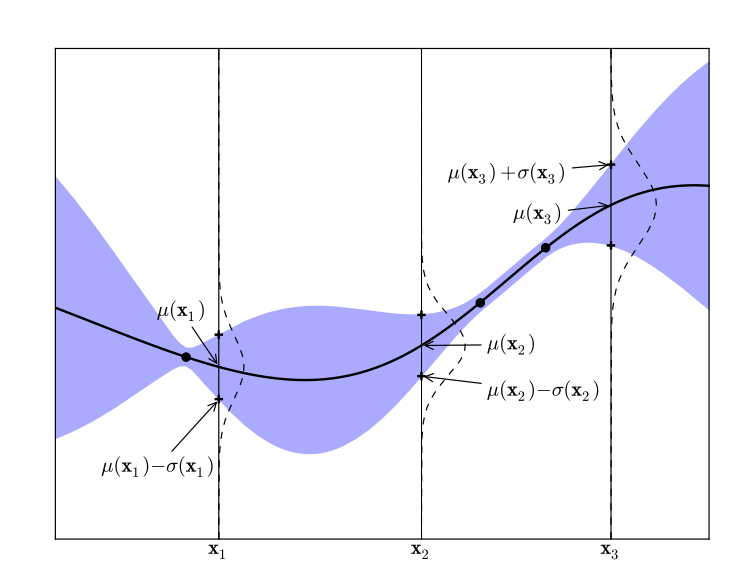
\includegraphics[width=1.0\textwidth]{images/gp-1d.png}
		\caption{A GP regression fit to three data points in 1D, shown as small black circles. The black line signifies the mean prediction, while the purple filled area shows one standard deviation at each point. The three points marked as $x_1, x_2, x_3$ are where we are computing the posterior, that is $p(x_1, x_2, x_3 | \mathcal{D})$. These points together have a multivariate Gaussian distribution, with a marginal 1D distribution shown vertically at each point. In order to draw a plot like this one we compute the posterior over a fine grid on the $X$ axis, and plot the mean parameter and the diagonal of the covariance matrix, giving us the standard deviation. Image source: \cite{nando-bopt-tutorial}.}
		\label{figure:gp-regression-1d}
	\end{center}
\end{figure}

By convention, we assume that the prior mean is a constant zero function, that
is $m(\vx) = 0$. Since the data is often normalized in practice, this does not
reduce the flexibility of the model. The power of a GP comes from its
covariance function, which for any two points $\vx_i$ and $\vx_j$ defines their
covariance $\kappa(\vx_i, \vx_j)$. If $\vx_i$ and $\vx_j$ have a high covariance,
the values of the function at those points will be similar.

\autoref{figure:gp-regression-1d} shows an example of a GP regression in one dimension. Because GP is a non-parametric model, it uses the whole dataset $\mathcal{D}$ in order to compute the posterior parameters. A theoretical benefit of this approach, as compared to using a parametric model like a random forest, is that we reduce the number of ways our model can underfit or overfit the data. Because we assume the mean to be zero, our only parameter is the kernel function $\kappa$. As we will explain later in \autoref{section:kernels}, we restrict ourselves even further to the Mat\'ern covariance function, which only has two hyperparameters.

Because the model is non-parametric, it can still fit any arbitrary dataset it is given, but its flexibility in terms of overfitting is controlled only via the kernel parameters. As an added benefit we can visualize the change in kernel parameters over time during Bayesian optimization in order to get further insight into how the model is fitting the data, as shown in \autoref{section:kernel-parameter-visualization}.

Intuitively, it is often useful to think of a GP as a function, which instead
of returning a scalar $f(x)$ returns the mean and standard deviation of a
Gaussian distribution over the possible values, centered at $x$. We leave a formal
treatment of GPs until \autoref{chapter:gp}.


% Bayesian optimization does not require any particular form of the prior
% distribution $p(f)$. We only need to have the ability to optimize the
% acquisition function to find the next sampling point $x$. In order to compute
% the acquisition function, we also need to have the ability to compute the
% posterior distribution $p(f|x)$. And as is the case with any other bayesian method,
%
%
% The prior distribution $p(f)$ allows the model to estimate
% the behavior of the function when data is lacking, but when more data becomes
% available, the likelihood overwhelms the prior during the posterior update
%
% Bayesian optimization is a sequential model-based approach to 
%
%
% In order to compute the posterior distribution $p(f|x)$ over functions, we need

\section{Hyperparameter versus Architecture Search}
\label{section:architecture-search}

Using our earlier definition, any parameter which the model does not learn on
its own could be considered a hyperparameter. This definition is broad enough
to allow a lot of flexibility, but some hyperparameters are better for the
framework of Bayesian optimization than others. Discrete and categorical
hyperparameters require special consideration. Bayesian optimization itself is
flexible in the sense that it allows for an arbitrary probabilistic model, but
the specific choice does matter when we consider discrete values. In the case
of GPs, the model itself has the ability to directly work with nothing
but continuous real-valued vectors.

There has been some recent work \citep{integer-valued-gp} showing better
approaches for handling integer-valued variables. The authors suggest to
round the appropriate values before computing their covariance. As the
kernel will consider the values as equivalent, their covariance will be maximized,
and the GP will be forced to predict a constant value over each integer region.
While this approach does help a little bit with integer-valued variables, it
does not improve handling of categorical (nominal) variables, which lack any form of
ordering. If we simply treat them as integers, the GP prior will enforce
relationships which do not exist.

An alternative approach to solving the problem with categorical variables is to
use a different model than GPs, namely random forests
\citep{nando-bayesian-out-of-the-loop}. Their main advantage is the ability to
naturally handle various types of data. We however do not explore random
forests in this work, as many of the hyperparameters of interest when tuning
neural networks are either continuous or integer-valued. Categorical variables,
such as activation functions, are better suited to be tweaked as part of neural
architecture search \citep{nasnet}.

Regardless of the probabilistic model, categorical variables cause many
immediate problems.  Consider the choice between SGD with momentum
\citep{overview-of-sgd} and Adam \citep{kingma2014adam}.  While SGD with
momentum has a \emph{momentum} hyperparameter, Adam does not, but it has its
own two extra hyperparameters, $β₁$ and $β₂$. This gives us two different sets
of mutually exclusive hyperparameters. Bayesian optimization however does not
have any natural way of handling problems like this. Even if we did externally
enforce two different modes based on which categorical values was chosen, it
would essentially be the same as running two experiments in parallel, one with
SGD, and one with Adam. Another issue arises in visualization, which is one of
the goals of this work. Inspecting the samples from two or more different modes
of the network at once is challenging at best, and with multiple categorical
variables the problem grows exponentially.

For these reasons, we chose not to provide direct support for categorical
variables, apart form converting them to integer variables with ordering and
treating them as such. Some categorical variables can be optimized by simply
treating them as fixed within a particular experiment, and then running
multiple instances of that experiment with a different value each. Other
categorical variables, such as the types of layers, activation functions, or
even the connections between modules, are better left for the framework of
neural architecture search, which treats them in a principled way.


\section{Related work}

There are a few notable mentions of related work in the area of tuning
hyperparameters of neural networks. The main motivation for this work is
Google Vizier \citep{google-vizier}, which is a proprietary service at Google
used for black box optimization. There also exist a few implementations of
Bayesian optimization. Spearmint \citep{spearmint} is the most fully featured
one, but comes with a very restrictive license, and does not perform any
visualization of the results. GPyOpt \citep{gpyopt2016}, RoBO \citep{robo} and scikit-optimize
\citep{scikit-optimize} are the most notable libraries for Bayesian
optimization, but they only provide the basic optimization loop for Bayesian
optimization, and do not handle long running experiments in a possibly
distributed environment.

An important mention is the \cite{automl}, which is an attempt at automating many aspects of Machine Learning. Several different approaches are being tried, for example the TPOT \citep{tpot} library uses evolutionary algorithms to not only tune hyperparameters, but also perform architecture search on Scikit-Learn algorithms, including building feature pre-processing pipelines, dimensionality reduction, and feature elimination.

Unfortunately, a commonly shared problem of these higher level approaches is the explosion of the search space. The more of the ML problem is handed over to the search procedure, the bigger the search space gets, and at some point one has to make certain trade-offs. The benefit of libraries as TPOT is their ease of use on small problems, where the model can be trained within a few minutes. But as is the goal of this thesis, we are interested in tuning hyperparameters of models which can take hours or even days to train, and in such case we want to be as efficient as possible.

Commercial services are also becoming more and more popular, both for AutoML and just for hyperparameter optimization. Apart from the Google Vizier service \citep{google-vizier} there also exist others, for example SigOpt \citep{sigopt} provides a cloud based solution to hyperparameter tuning using Bayesian optimization. Amazon SageMaker \citep{amazon-sagemaker} is yet another commercially available cloud based hyperparameter tuning service based on Bayesian optimization.



